\subsection{Component Identification in Figure T-3}
\label{T6C11}

\begin{tcolorbox}[colback=gray!10!white,colframe=black!75!black,title=T6C11]
What is component 4 in figure T-3?

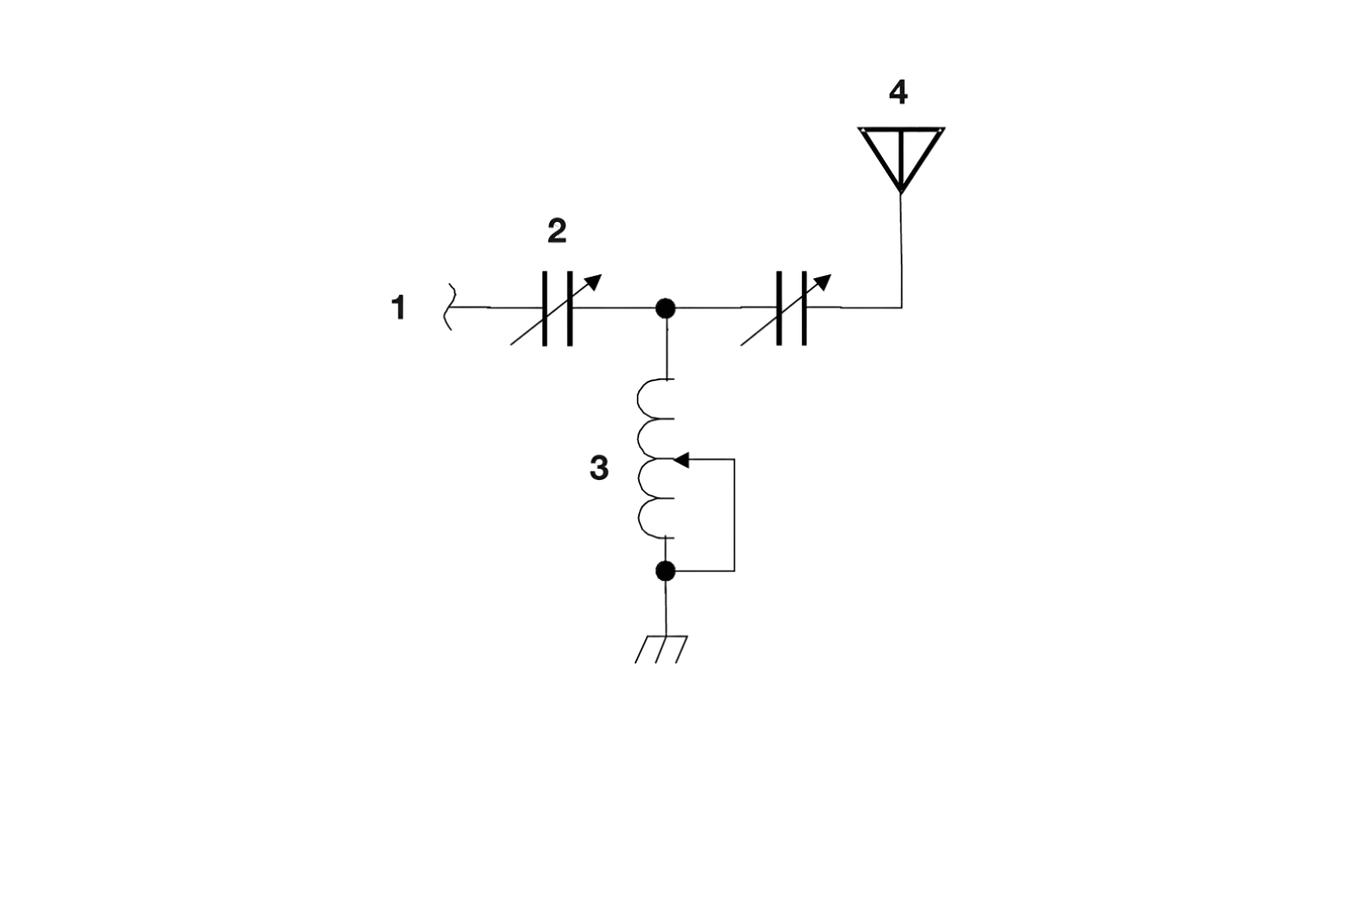
\includegraphics[width=0.5\textwidth]{tech/images/t3.png} 

\begin{enumerate}[label=\Alph*)]
    \item \textbf{Antenna}
    \item Transmitter
    \item Dummy load
    \item Ground
\end{enumerate}
\end{tcolorbox}

\subsubsection{Intuitive Explanation}
Imagine you’re playing a game of catch with a friend. You throw the ball (that’s the transmitter), and your friend catches it (that’s the antenna). In this case, component 4 is like your friend’s hands—it’s the antenna that catches the radio waves. So, the correct answer is the antenna. Easy, right?

\subsubsection{Advanced Explanation}
In radio communication systems, the antenna (component 4 in figure T-3) is a crucial element that converts electrical signals into electromagnetic waves for transmission and vice versa for reception. The transmitter generates the signal, but it’s the antenna that radiates this signal into the air. The dummy load is used to absorb power without radiating it, and the ground is a reference point in the circuit. Therefore, the correct identification of component 4 is the antenna.

% Prompt for diagram: Generate a diagram showing a radio communication system with labeled components, including the antenna, transmitter, dummy load, and ground.